%TODO synthèse
%TODO glossaire et bibliographie etc ..

%%%%%%%%%%%%%%%%%%%%%%%%%%%%%%%%%%%%%%%%%%%%%%%%%%%%%%%%%
%                      Préambule                        %
%%%%%%%%%%%%%%%%%%%%%%%%%%%%%%%%%%%%%%%%%%%%%%%%%%%%%%%%%

%%%%%%%%%%%%%%%%%%%%%%%%%%%%%%%%%%%%%%%%%%%%%%%%%%%%%%%%%%%%%%%%%
%                      Préambule type                          %
%%%%%%%%%%%%%%%%%%%%%%%%%%%%%%%%%%%%%%%%%%%%%%%%%%%%%%%%%%%%%%%%



\def\changemargin#1#2{\list{}{\rightmargin#2\leftmargin#1}\item[]}
\let\endchangemargin=\endlist 

%%%%%%%%%%%%%%%%%% Classe dudit Document %%%%%%%%%%%%%%%%%%%%%%%
\documentclass[a4paper,12pt,openany]{report} % sert à définir des propriétés e base sur les articles
% Autre paramètres connnus: 	*book => pour de vrais livres
%				*article pour des artiles dans des revues scientifiques, des présentations, des rapports courts, des documentations, des invitation etc....
%				*report por des rapports plus long contenant plusieurs chapitres, des petits livres, des thèses
%				*Slides pour des transparants
%				*foiltex
% Option: Xpt taille de la police,  4apaper/letterpaper/a5paper/b5paper/executivepaper, fleqn, leqno, titlepage/notitlepage indique si une nouvelle page doit être commencée après le titre du document, twocolumn,twoside/oneside,



%%%%%%%%%%%%%%%%%%%%%%%% Package %%%%%%%%%%%%%%%%%%%%%%%%%%%%%%%
\usepackage{doc}% permet de documenter des programmes (cf doc.dtx]
\usepackage{exscale} % fournit des version de taille de caractère que LaTeX va utiliser (cf ltexscale.dtx)
\usepackage{fontenc} % spécifie le codage des police de caractère que LaTeX va utiliser (cf ltoutenc.dtx)
%\usepackage[latin]{inputenc} %Autorise les caractères acentués
\usepackage{ifthen} % fournit des commandes de conditions (cf ifthen.dtx)
\usepackage{latexsym} %permet l'utilisation de la police des symboles LaTeX
\usepackage{makeidx} %fournit des commandes pour réaliser un index
\usepackage{syntonly} % analyse le doc sans le formater
\usepackage[T1]{fontenc}
\usepackage[utf8x]{inputenc} 
%\usepackage[utf8]{inputenc}% permet de spécifier le codeage des caractère utiliser dans le source.
\usepackage[english,francais]{babel}
%\usepackage{asmath} %Fonctions servant à l'écriture mathématique
\usepackage{xspace} %Fonctions permettant d'introduire des espaces
\usepackage{xargs} %Permet d'utiliser de définir plus simplement des fonctions
\usepackage{trace}%Permet d'utiliser des traces de debbug
\usepackage{show2e}% debbug
\usepackage[pdftex]{graphicx}
\usepackage{hyperref}

%%%%%%%%%%%%%%%%% Style du pied de page %%%%%%%%%%%%%%%%%%%%%%%%

\pagestyle{plain}% imprime le numéro de page au milieu du pied de page
%\pagestyle{heading}%imprime le titre du chapitre courant et le numéro dans l'en tête et laisse le pied de page vide.
%\pagestyle{empty}% laisse l'en tête et le pied de page vide


%Nota bene: On peut changer le pied de page en court en utilisant \thispagestyle


%%%%%%%%%%%%%%%%% Césure   %%%%%%%%%%%%%%%%%%%%%%%%

\hyphenation{FORTRAN}
\hyphenation{An-ti-cons-ti-tu-tion-nel-le-ment}

%%%%%%%%%%%%%%%% Citation Environement %%%%%%%%%%%%

\newsavebox{\nomepigraphe}
\newenvironment{epigraphe}[1]
	{% clause begin
	\vspace*{-1.5cm}%
	\small\sffamily% mise en évidence
	\savebox{\nomepigraphe}{#1}% une boîte pour sauvegarder
	% l’ origine de la citation
	\slshape% tout est penché
	\begin{changemargin}{0pt}{-2cm}% on se met au large
	\begin{flushright}}% tout est poussé à droite
	{% clause end
	\\[4pt]\usebox{\nomepigraphe}.% insertion de l’origine
	\end{flushright}%
	\end{changemargin}\par\vspace*{0.6cm}}

%
\input ./preambule.tex %sans saut de ligne


%%%%%%%%%%%%%%Titre%%%%%%%%%%%%%%%%%%%%%%%%%%%%%%%%%%%%
\title{ Projet de 3 année à l'INSA Centre Val de Loire } % Titre du document
\author{BAIZ Mamoune && BAIZ Mamoune} % Auteur
\date{\today} % Date de création


%%%%%%%%%%%%%%%%%%%%%%%Debut Doc%%%%%%%%%%%%%%%%%%%%%%%
\begin{document} % Début du document
%%%%%%%%%%%%%%%%%%%%%%Page de Garde%%%%%%%%%%%%%%%%%%%%
{
\begin{titlepage}
  \begin{sffamily}
  \begin{center}

    % Upper part of the page. The '~' is needed because \\
    % only works if a paragraph has started.
    
\includegraphics[scale=0.5]{Images/png/insa_logo.png}~\\[1.5cm]

    \textsc{\LARGE Institut National des Sciences Appliquées  Centre Val de Loire }\\[2cm]

    \textsc{\Large Rapport de projet 3\up{ème} année option 2SU}\\[1.5cm]

    % Title
%    \HRule \\[0.4cm]
    { \huge \bfseries Domotique\\[0.4cm] }

%    \HRule \\[2cm]
    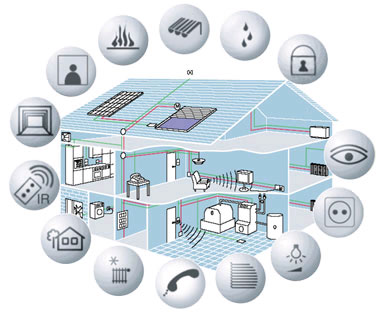
\includegraphics[scale=0.5]{Images/jpg/domotic.jpg}
    \\[2cm]

    % Author and supervisor
    \begin{minipage}{0.4\textwidth}
      \begin{flushleft} \large
        BAIZ Mamoune et MUNIER Marc \\
        Promo 2016\\
      \end{flushleft}
    \end{minipage}
    \begin{minipage}{0.4\textwidth}
      \begin{flushright} \large
        \emph{Encadrant :} M. Briffaut\\
      \end{flushright}
    \end{minipage}

    \vfill

    % Bottom of the page
    {\large 9 Février 2016}

  \end{center}
  \end{sffamily}
\end{titlepage}
}
%%%%%%%%%%%%%%%%%%%%%%%Page Vierge%%%%%%%%%%%%%%%%%%%%
\newpage



%%%%%%%%%%%%%%%%%%%%% Remerciment %%%%%%%%%%%%%%%%%%%%
\newpage
\section*{Remerciement}
Je tiens à remercier Mr Briffaut pour sa investissement 
%TODO
\clearpage
%%%%%%%%%%%%%%%%%%%%%Résumé%%%%%%%%%%%%%%%%%%%%%%%%%%%
\section*{Résumé}
Ce rapport présente mon travail et les enseignements acquis lors de mon stage de deuxième année d'école d'ingénieurs au seins du Centre technique de la Gendarmerie nationale. 

Ce centre technique acceuille en ces lieux le service de traitement de l'information de la Gendarmerie (STIG). Ce service a pour vocation de garantir la continuité des applications, l'intégrité et la confidentialité de données sensibles. L'enjeux de ces vocations est cruciale dans un milieu tel que la gendarmerie. En effet, les applications hébergées par ce service peuvent sauver des vies humaines. Et de part cette raison, on peut tout à fait comprendre que la sécurité informatique soit une priorité pour le STIG.

C'est pourquoi en 2014, le STIG crée un nouveaux groupe chargé de la sécurité opérationelle.Ce groupe est composé de quatres gendarmes de carrières et est dirigé par le Lieutenant Dubois, officier de gendarmerie possédant un diplome d'ingénieur délivré par l'école nationale supérieur de Bourges (ENSIB).

La mission qui m'a été confiée, fut d'automatiser la détection d'évènement de sécurité dans l'historique des événments survenus dans les différents serveurs du STIG. Concrétement mon projet se résume à l'élaboration d'un outil informatique qui préviendrait les autorités compétantes lors d'évènement mettant en cause la sécurité du Service.

C'est au travers de deux mois de stage et de projets que j'ai pu finalement proposer une version, non définitive mais fonctionnelle de cet outil informatique.
%%%%%%%%%%%%%%%%%%%%%table des matières%%%%%%%%%%%%%%%
\newpage
\tableofcontents
\clearpage
%%%%%%%%%%%%%%%%%%%%%%%%%%%%%%%%%%%%%%%%%%%%%%%%%%%%%%
\section{Introduction}
Dans le cadre de ma formation d'ingénieur spécialisé dans la sécurité et les technologies informatiques à l'INSA centre val de Loire, j'ai eu la possibilité de réaliser un stage de deux mois. J'ai effectué ce stage au sein de la gendarmerie nationale. Il fait suite à ma deuxième année dans le cursus ingénieur.

Dans ce rapport, je vous présenterai brièvement la gendarmerie nationale puis l'apport de mon stage dans cette institution nationale.
\section{Présentation de l'entreprise}
\subsection{Histoire de la Gendarmerie Nationale}
La Gendarmerie Nationale est l'héritière des traditions et coutumes de la maréchaussée. La maréchaussée était une institution de l'état composée de militaires plus disciplinés que les autres. Les autorités compétentes de l'époque lui avaient attribué comme mission de contrôler et surveiller les autres militaire, qui étaient alors plus débandés et pillards. Cette mission s'est peu à peu étendue à l'ensemble de la population et à l'ensemble du territoire national. Pour répondre à cette nouvelle prérogative, la maréchaussée crée en 1720 les brigades. Ce sont des unités organiques répandues à travers le territoire national.

En 1791, sous l'autorité du Directoire, la maréchaussée prit l'appellation de Gendarmerie Nationale. Elle perdit par la même occasion ses fonctions de justice prévôtale.

\end{document}
